%%%%%%%%%%%%%%%%%%%%%%%%%%%%%%%%%%%%%%%%%%%%%%%%%%%%%%%%%%%%%%%%%%%%%%%%%%%%%%%%
%2345678901234567890123456789012345678901234567890123456789012345678901234567890
%        1         2         3         4         5         6         7         8

\documentclass[letterpaper, 10 pt, conference]{ieeeconf}  % Comment this line out if you need a4paper

%\documentclass[a4paper, 10pt, conference]{ieeeconf}      % Use this line for a4 paper

\IEEEoverridecommandlockouts                              % This command is only needed if 
                                                          % you want to use the \thanks command

\overrideIEEEmargins                                      % Needed to meet printer requirements.

%In case you encounter the following error:
%Error 1010 The PDF file may be corrupt (unable to open PDF file) OR
%Error 1000 An error occurred while parsing a contents stream. Unable to analyze the PDF file.
%This is a known problem with pdfLaTeX conversion filter. The file cannot be opened with acrobat reader
%Please use one of the alternatives below to circumvent this error by uncommenting one or the other
%\pdfobjcompresslevel=0
%\pdfminorversion=4

% See the \addtolength command later in the file to balance the column lengths
% on the last page of the document

% The following packages can be found on http:\\www.ctan.org
%\usepackage{graphics} % for pdf, bitmapped graphics files
%\usepackage{epsfig} % for postscript graphics files
%\usepackage{mathptmx} % assumes new font selection scheme installed
\usepackage{times} % assumes new font selection scheme installed
\usepackage{amsmath} % assumes amsmath package installed
\usepackage{amssymb}  % assumes amsmath package installed
\usepackage{tikz} 
\usepackage{pgfplots}


\usetikzlibrary{automata,positioning,arrows}


\title{\LARGE \bf
% Preparation of Papers for IEEE Sponsored Conferences \& Symposia*
Modeling Market Making as a Markov Decision Process
}

\author{Franklin Glance}

\begin{document}



\maketitle
\thispagestyle{empty}
\pagestyle{empty}


%%%%%%%%%%%%%%%%%%%%%%%%%%%%%%%%%%%%%%%%%%%%%%%%%%%%%%%%%%%%%%%%%%%%%%%%%%%%%%%%
\begin{abstract}

This project focuses on the application of the Avellaneda-Stoikov (AS) pricing model for market making in a high frequency trading environment, by modeling the market making problem as a Markov Decision Process (MDP). Using level 10 order book data for several stocks over a trading day, we simulated the implementation of the AS strategy as an MDP, and evaluated its performance based on the goals of providing liquidity and managing inventory risk. The model didn't yield direct profitability, however it provided great insight into the dynamics of market microstructure and managed inventory risk. Although limited by certain idealized assumptions of the AS strategy and the exclusion of transaction fees, this project successfully models the market making problem as an MDP, and utilizes the closed form pricing model developed by Avellaneda-Stoikov to effectively perform market making. It lays the groundwork for further research in algorithmic trading, and highlights the potential for utilizing the MDP model as a framework for developing more sophisticated market making strategies.   

\end{abstract}


%%%%%%%%%%%%%%%%%%%%%%%%%%%%%%%%%%%%%%%%%%%%%%%%%%%%%%%%%%%%%%%%%%%%%%%%%%%%%%%%
\section{INTRODUCTION}
Market making plays a crucial role in financial markets by providing liquidity to participants and ensuring that markets are efficient. Market makers are always ready to buy and sell securities at any time, earning profit from capturing the bid-ask spread while bearing risk associated with holding inventory positions. In recent years, the growing complexity of financial markets has led to the development of automated market making strategies. These strategies use algorithms to automatically place orders in the market, and are able to respond to changing market conditions in real time. 

One potential approach to designing such strategies is to model the market making problem as a Markov Decision Process (MDP), a widely used mathematical framework for modeling sequential decision-making problems. When formulated as an MDP, the market making decision process consists of placing orders in the market based on information gleaned from historical market data.

In this paper, we focus on the Avellaneda-Stoikov market making model, a well-known strategy that dynamically adjusts bid and ask prices in response to market information such as asset price, order book state, volatility, and trading intensity. The Avellaneda-Stoikov model seeks to maximize expected profit from the bid-ask spread, while minimizing risk from holding large inventory positions. 


\section{LITERATURE REVIEW}

The literature on market making is vast and spans many decades, encompassing a wide range of theoretical and empirical approaches to market making. In this section, we briefly review some of the most relevant papers on market making, with a focus on the Avellaneda-Stoikov model.

\subsection{Classic Market Making Models}
One of the first papers on classic market making is "The Supply of Dealer Services in Securities Markets" (Stoll 1978 \cite{c1}). The paper discusses the function of dealers in equity securities markets, the efficiency of different methods of providing dealer services and the regulatory constraints under which dealers should operate. The paper aims to develop a more explicit and rigorous model of the individual dealer and to discuss the implications for the cost of trading of different market organizations of dealers. They model the market maker as a monopolist who sets bid and ask prices to maximize expected profit.
Another fundamental paper, “Market microstructure” by Mark B. Garman was published in the Journal of Financial Economics in 1976 \cite{c2}. The paper assumes that a collection of market agents can be treated as a statistical ensemble and their market activities are depicted as the stochastic generation of market orders according to a Poisson process. The paper's objective was to effectively describe the ‘temporal microstructure’, or moment-to-moment trading activities in asset markets. If the moment-to-moment trading activities can be modeled, then market makers can efficiently make markets. These early models laid the groundwork for subsequent research by providing the basis for stochastic modeling and simulation of market making. 

\subsection{Inventory Models and Information Assymetry}
Building on these early studies, Ho and Stoll (1981)\cite{c3} introduced an inventory model that incorporated information asymmetry between market makers and informed traders. Their model demonstrates that market makers adjust bid-ask spreads to account for both inventory risk and the risk of trading with better-informed counterparties. This builds on the monopolistic model from Stoll's earlier work, and is a closer model to real world market conditions. Glosten and Milgrom (1985)\cite{c4} further extended this line of research by developing a model in which market makers learn from the order flow and update their beliefes about the true value of the asset, resulting in dynamically adjusting bid-ask spreads.

\subsection{Optimal Market Making Strategies}
Avellaneda and Stoikov (2008)\cite{c5} proposed a market making model that significantly influenced further research in the field. Their model, kown as the Avellaneda-Stoikov model, is an optimal market making strategy that dynamically adjusts bid and ask prices based on market information such as asset price, order book state, volatility, and trading intensity. The Avellaneda-Stoikov model seeks to maximize expected profit from the bid-ask spread, while minimizing risk from holding large inventory positions. The closed form solution for bid-ask pricing provided in this paper is an efficient means of determining optimal bid and ask prices in real time, and will be used as the basis for decision making in our MDP.  



\section{METHODS}

In this section, we provide an overview of the method for simulating the implementation of the Avellaneda-Stoikov pricing model as a Markov Decision Process (MDP) on level 10 order book data for AAPL, AMZN, GOOG, INTC, and MSFT for the day of 2012-06-21. 

\subsection{Data Preparation}

We started by obtaining level 10 order book data for AAPL, AMZN, GOOG, INTC, and MSFT from LOBSTER \cite{c6}. This data contained bid and ask prices and volumes for 10 levels of the order book, as well as the time of each update. This data is crucial for accurately simulating high frequency market making in a limit order book. We preprocessed the raw data to compute relevant metrics for the MDP, specifically the volatility and trading intensity. We used a rolling indicator with a window size of 100 and 200 seconds to compute the volatility and trading intensity, respectively.

\subsubsection{Computing Trading Intensity}

In order to take into account the microstructure of financial markets, it is critical to incorporate information regarding the intensity with which a given limit order will be executed at a given price. This metric can be estimated as a Poisson intenisty $\lambda$ with which a limit order will be executed as a function of its distance $\delta$ to the mid-price. In simple terms, $\lambda(\delta)$ represents the expected rate at which orders arrive $\delta$ distance away from the current mid price, and is directly tied to the transition probabilities in our MDP formulation discussed later. The derivation in Avellaneda and Stoikov (2008) \cite{c5} produces the following formula for the trading intensity as a function of $\delta$: $$\lambda(\delta) = A \exp(-k*\delta)$$ 

We chose to use 5 price levels to compute the trading intensity. This means that we computed a $\lambda$ value 10 times, 5 for prices above the mid-price and 5 for prices below the mid-price. The AS model is built of of non-directional computation of order flow, however further studies should consider the effect of providing directional order intensity information to the model. The parameters $k$ and $A$ capture the shape of the trading intensity curve, and are defined as follows:
\begin{align}
        k &= \mathbb{E}_{P1,P2}\left(\frac{\log \lambda(\Delta P1) - \log \lambda(\Delta P2)}{\Delta P1 - \Delta P2}\right) \\ 
        A &= \mathbb{E}_{P}\left(\lambda(\Delta P)\exp(k*\Delta P)\right)
\end{align}

Estimating $A$ and $k$ requires fitting a linear regression model to the data. We used \texttt{scipy.curve\_fit} to fit a linear regression model to the data at each time step, and used the resulting coefficients to compute the trading intensity at each time step. The curve fitting can be thought of as fitting a curve to the price levels, where the curve height represents the likelihood (rate) of an order being filled at a given price level. After being fit, the curve looks similar to the one shown in Figure \ref{fig:trading_intensity}.
\begin{figure}[h]
        \centering
        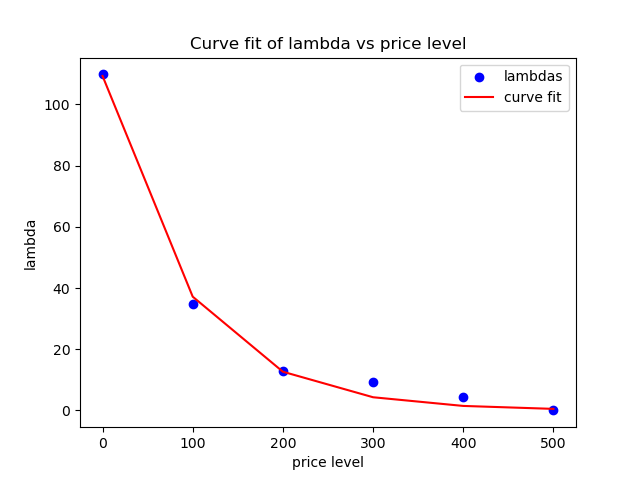
\includegraphics[width=0.5\textwidth]{trading_intensity.png}
        \caption{Trading intensity curve}
        \label{fig:trading_intensity}
\end{figure}
As mentioned earlier, the equation of the curve fit line is $\lambda(\delta) = A*\exp(-k*\delta)$, where $A$ and $k$ are the coefficients of the linear regression model. The coefficient $k$ is the kappa value used in the MDP. $k$ captures the shape of the curve, so larger $k$ values represent a lower likelihood of an order being filled at price levels further from the mid-price. $A$ is the alpha value used in the MDP. $A$ represents the maximum likelihood of an order being filled at the mid-price, and is not needed for the MDP. 

When modeling as an MDP, the trading intensity represents the likelihood of transitioning to an "order filled" state, given the current ask and bid prices. 

\subsection{MDP Formulation}
We formulated the market making problem as an MDP, which consistes of the following components:
\begin{itemize}
        \item \textbf{State space:} The state at time $t$ is a tuple $(S_t, q_t, k_t, \sigma^2_t, r_t)$, where here $S_t$ is the mid-price, $q_t$ is the current inventory position, $k_t$ is the trading intensity, and $\sigma^2_t$ is the price volatility at time $t$. 
        \item \textbf{Action space:} The action space consists of placing bid and ask orders in the limit order book. Specifically, and action $a\in A$ is a tuple $(p_a, p_b, v_a, v_b)$ representing the bid and ask prices and volumes. The market maker must choose the optimal values for $p_a, p_b, v_a, v_b$ given the current state.
        \item \textbf{Transition probabilities:} The transition probabilities are the likelihood of moving from one state to another, given a particular action. In our simulation, these probabilities are estimated using the level 10 order book data and the Poisson process assumption for order arrivals. This probability is captured in the trading intensity parameter $k$. These probabilities are used when determining the optimal action, by placing bid and ask orders at prices with higher likelihood of being filled. The likelihood value is given by $\lambda(\delta)$, where $\delta$ is the distance from the mid-price.
        \item \textbf{Reward function:} The reward function is defined as the profit obtained from executing the bid or ask orders, taking into account both the bid-ask spread and the potential inventory risk. The objective is to maximize the expected cumulative reward over the trading day. This reward function is optimized in its closed form using the Avellaneda-Stoikov pricing strategy.
\end{itemize}

Due to the time-series nature of market data, a closed form solution to the MDP is not possible. However, the Avellaneda-Stoikov pricing strategy combined with an intuitive inventory management algorithm provides a computationally efficient means of determining optimal bid and ask prices in real time.

\subsection{Avellaneda-Stoikov Pricing Strategy}
Avellaneda-Stoikov market making involves 3 main steps:
\begin{enumerate}
        \item Determine the optimal bid and ask prices for the given security based on market information (asset price, order book, volatility, and trading intensity).
        \item Dynamically adjust bid and ask prices in response to changing market conditions. These adjustments are aimed at reducing the risk of holding large inventory positions and maximizing profit from the bid-ask spread.
        \item Adjust bid and ask volume to manage inventory (ideally keeping position at 0).
\end{enumerate}

The formulation can be expressed as an optimization problem, where the goal is to maximize $$u(s,x,q,t) = \mathbb{E} \left[e^{-\gamma(X_t+q_t*S_t)} \right]$$
where $\delta^a, \delta^b$ are the predicted bid-ask spreads, $\gamma$ is the risk aversion parameter, $X_T$ is wealth at time $t$, $q_t$ is the inventory position at time $t$, and $S_t$ is the mid price at time $t$. 

A bid or ask order is filled if the order book price reaches the limit price. The likelihood of an order arriving at a given price level in the order book is modeled as a Poisson proccess with rate $\lambda_i$, where $i$ is the market depth. In short, the likelihood of an order being filled is both dependent on the market depth (distance from the midpoint price), and the rate of order arrivals at the given depth. In the Avellaneda-Stoikov model, the rate of order arrivals at different price levels is captured by the trading intensity parameter $k_t$. Given $S_t$, $q_t$, $k_t$, and $\sigma^2_t$, the optimal bid and ask spread ($\delta^a_t, \delta^b_t$) are given by:
\begin{align*}
        r(t) &= S_t - q_t * \gamma * \sigma^2_t \rightarrow \text{indifference price} \\
        \delta^a_t + \delta^b_t &= \gamma*\sigma^2_t + \ln(1+\frac{\gamma}{k_t}) \rightarrow \text{bid-ask spread} \\
\end{align*}
Given the indifference price and bid-ask spread, the optimal bid and ask prices can be calculated by adding and subtracting half the bid-ask spread from the indifference price. 
\begin{align*}
        \text{bid price} &= r(t) - \frac{\delta^a_t}{2} \\
        \text{ask price} &= r(t) + \frac{\delta^b_t}{2}
\end{align*}
The state diagram contains 3 main "states": Quoting (Q), Waiting for Bid Fill (Wb), Waiting for Ask Fill (Wa), and Caputured Spread (S). The state diagram along with transition probabilities is shown in Figure \ref{fig:mdp_diagram}. The transition probabilities are estimated based on the action taken in each state (bid price, ask price and volume), and the definitions are shown in Table \ref{tab:mdp-definitions}.        
\begin{figure}[h!]
        \centering
        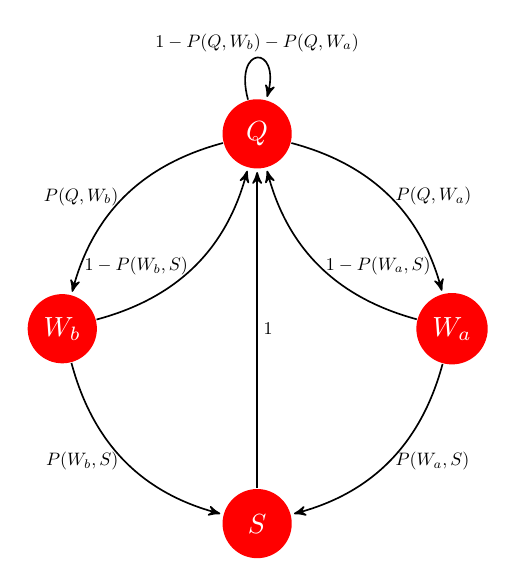
\begin{tikzpicture}[->,>=stealth',shorten >=1pt,auto,node distance=3.5cm,
                semithick]
        \tikzstyle{every state}=[fill=red,draw=none,text=white]
        
        \node[state]         (Q)              {$Q$};
        \node[state]         (W_b) [below left of=Q] {$W_b$};
        \node[state]         (W_a) [below right of=Q] {$W_a$};
        \node[state]         (S) [below right of=W_b] {$S$};
        
        \begin{scope}[every node/.style={scale=.65}]
        
        \draw (Q) edge [bend right] node [left] {$P(Q,W_b)$} (W_b);

        \draw (Q) edge [bend left] node [right] {$P(Q,W_a)$} (W_a);
        \draw (W_b) edge [bend right] node [left] {$P(W_b,S)$} (S);
        \draw (W_a) edge [bend left] node [right] {$P(W_a,S)$} (S);
        \draw (S) edge [] node [right] {$1$} (Q);
        \draw (W_b) edge [bend right] node [left] {$1-P(W_b,S)$} (Q);
        \draw (W_a) edge [bend left] node [right] {$1-P(W_a,S)$} (Q);

        \draw (Q) edge [loop above] node {$1-P(Q,W_b)-P(Q,W_a)$} (Q);



        \end{scope}

        
        \end{tikzpicture}
        \caption{Markov chain for the Avellaneda-Stoikov model.}
        \label{fig:mdp_diagram}
\end{figure}


% Please add the following required packages to your document preamble:
% \usepackage{graphicx}
\begin{table}[h!]
        \centering
        \caption{}
        \label{tab:mdp-definitions}
        \resizebox{\columnwidth}{!}{%
        \begin{tabular}{l|l|l}
         & Definition & Description \\ \hline
        $p_a, p_b$ & ... & Chosen Bid and Ask prices \\
        $P(Q,W_b)$ & $\lambda(p_a)$ & Likelihood of ask fill \\
        $P(Q, W_a)$ & $\lambda(p_b)$ & Likelihood of bid fill \\
        $P(W_b, S)$ & $\lambda(p_b)$ & Likelihood of bid fill \\
        $P(W_a, S)$ & $\lambda(p_a)$ & Likelihood of ask fill \\
        $R(S)$ & $p_a-p_b$ & Reward from capturing spread
        \end{tabular}%
        }
        \end{table}

\subsection{Inventory Management}

In any market making strategy, inventory management is a crucial aspect. Market makers, while providing liquidity, may accumulate positions in the security, thereby exposing themselves to risk due to price movements. In the real world, market makers hedge their positions which eliminates most downside risk. However, hedging becomes more costly as inventory positions accumulate. Therefore, it is essential to develop strategies that can help keep the inventory close to zero, effectively managing the inventory risk. 

In our project, we use a simple inventory management strategy that dynamically adjusts bid and ask sizes based on the current inventory level. Order size is given by the following equation: $$\phi_t^{bid} = \begin{cases}
        \phi_t^{max} & \text{ if } q_t \leq 0 \\
        \phi_t^{max} \cdot \exp(-\eta q_t) & \text{ if } q_t > 0
\end{cases} $$
$$ \phi_t^{ask} = \begin{cases}
        \phi_t^{max} & \text{ if } q_t \geq 0 \\
        \phi_t^{max} \cdot \exp(-\eta q_t) & \text{ if } q_t < 0
\end{cases} $$
where $\phi_t^{max}$ is the maximum order size, and $\eta$ is a parameter that controls the rate at which the order size decays as the inventory increases. The intuition behind this strategy is that as the inventory increases, the order size should decrease, and vice versa. The parameter $\eta$ controls the rate at which the order size decays. A higher value of $\eta$ implies that the order size decays faster as the inventory increases, and vice versa. A visualization of order size vs inventory is shown in Figure \ref{fig:order_size_vs_inventory}.

% plot of order size vs inventory
\begin{figure}
        \centering
        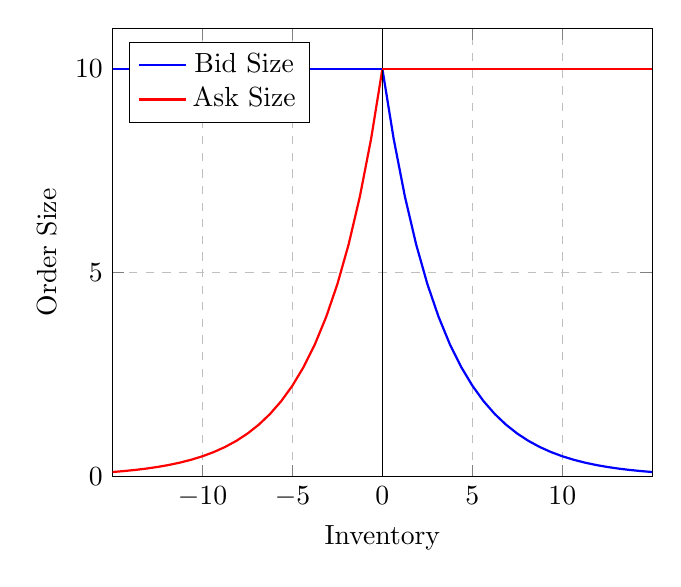
\begin{tikzpicture}
                \begin{axis}[
                        % title={Order Size vs Inventory, $\eta=0.3, \phi_t^{max} = 10$},
                        xlabel={Inventory},
                        ylabel={Order Size},
                        % position x label below graph
                        xmin=-15, xmax=15,
                        ymin=0, ymax=11,
                        xtick={-10,-5,0,5,10},
                        ytick={0,5,10},
                        legend pos=north west,
                        ymajorgrids=true,
                        grid style=dashed,
                        grid = major,
                ]
                \addplot [blue, thick, domain=0:15] {10*exp(-0.3*x)};
                \addlegendentry{Bid Size}
                \addplot [red, thick, domain=-15:0] {10*exp(0.3*x)};
                \addlegendentry{Ask Size}
                % add vertical line at x=0
                \draw (axis cs:0,0) -- (axis cs:0,11);
                \draw [blue, thick] (axis cs:-15,10) -- (axis cs:0,10);
                \draw [red, thick] (axis cs:0,10) -- (axis cs:15,10);
                \end{axis}
        \end{tikzpicture}
        \caption{Order size vs inventory for $\eta=0.3, \phi_t^{max} = 10$.}
        \label{fig:order_size_vs_inventory}
\end{figure}

\subsection{Simulation}
With these components defined, we can model the Avellaneda-Stoikov market making strategy as an MDP, and simulate the results of the strategy over a trading day. We ran the simulation in level 10 order book data for each stock. At each time step, we observe the current state and update the prices according to the Avellaneda-Stoikov model.

To simulate market order execution, we follow a series of steps designed to closely resemble the acutal process of executing market orders in a limit order book. The primary goal is to accurately capture the dynamics of order arrivals, order cancellations, and price movements. 

\begin{enumerate}
        \item \textbf{Initialize the limit order book:} At the beginning of the trading day, we initialize the limit order book using the level 10 order book data for each stock. The order book contains the best bid and ask prices, along with their corresponding volumes, for the top 10 levels on both sides of the book.
        \item \textbf{Iterate through time steps:} We iterate through the time steps (0.25s between updates) of the trading day, updating the state variables and applying the optimal policy derived from the MDP solution. At each time step, we simulate the arrival of new market orders and the cancellation of existing limit orders.
        \item \textbf{Market order arrivals:} We assume that market orders arrive according to a Poisson process with a time-varying arrival rate, which can be estimated from the trading intensity parameter $k_t$. For each time step, we generate a random number to determine whether a market buy or sell order arrives. If a market order arrives, we match it with the corresponding best limit order on the opposite side of the book. If the market order volume is greater than the available limit order volume at the best price, the order is executed in multiple steps, consuming liquidity from several levels of the book.
        \item \textbf{Order cancellations:} In addition to market order arrivals, we also simulate the cancellation of existing limit orders. We assume that order cancellations follow a stochastic process, which can be estimated from historical order book data. At each time step, we generate random numbers to determine whether any limit orders are canceled and, if so, update the order book accordingly.
        \item \textbf{Update inventory and wealth:} After simulating market order arrivals and order cancellations, we update the market maker's inventory position and wealth based on the executed bid and ask orders. The inventory position is updated by adding or subtracting the executed order volume, while the wealth is updated by accounting for the realized profits or losses due to the bid-ask spread and the potential inventory risk.
        \item \textbf{Update state variables:} Finally, we update the state variables, including the mid-price, trading intensity, and price volatility, using the updated order book data. The new state is used as input for the optimal policy at the next time step.
\end{enumerate}
By simulating market order execution in this manner, we emulate the behavior of real-world financial markets and gain a better understanding of the dynamics of the Avellaneda-Stoikov market making strategy under realistic market conditions. 
\subsection{Verification and Validation}
When simulating market data, Verification and Validation are crucial processes that ascertain the model's correctness and its ability to represent th real-world system accurately. Throughout our study, we followed a systematic approach to verify the implementation of our model and validate its performance using real world data. 

\textbf{Verification:} The verification process focused on ensuring that our model of the Avellaneda-Stoikov strategy as a Markov Decision Process (MDP) was implemented correctly. We used unit tests to verify that each python function computed the proper output, by hand-computing metrics such as the bid-ask spread, volume weighted average mid price, kappa, and volatility and comparing them to the function outputs. 

\textbf{Validation:} After verifying that our model was working properly, the validation process focused on evaluating the performance of the Avellaneda-Stoikov strategy under realistic market conditions. We used real-world order book data to simulate the execution of market orders and validate the performance of the strategy. We first checked the price data to ensure that it was consistent with the actual stock prices during the given timeframes. We then ran the simulation for each stock and compared the results to the actual bid-ask spread and volume weighted average mid price. We also compared the simulated trading intensity and volatility to the actual values. We performed a sensitivity analysis on the model hyper-parameters such as the risk aversion parameter and the sampling windows for intensity and volatility. 

Our rigorous verification and validation process ensured that our model was implemented correctly and that it can accurately represent the Avellaneda-Stoikov strategy under realistic market conditions.

\section{RESULTS}
Our application of the Avellaneda-Stoikov strategy, as modeled through a Markov Decision Process, provided insightful results that enhanced our understanding of the inherent complexities in market making, particularly in a high-frequency trading environment.

\subsection{Model Performance}

Our simulation of this strategy, applied to level 10 order book data for AAPL stock over a trading day, yielded an outcome wherein the model did not generate a net profit. The PnL is shown below in Figure \ref{fig:pnl}. While this might initially seem disappointing, it is essential to interpret these findings in the broader context of market making and algorithmic trading. 

\begin{figure}[h]
\centering
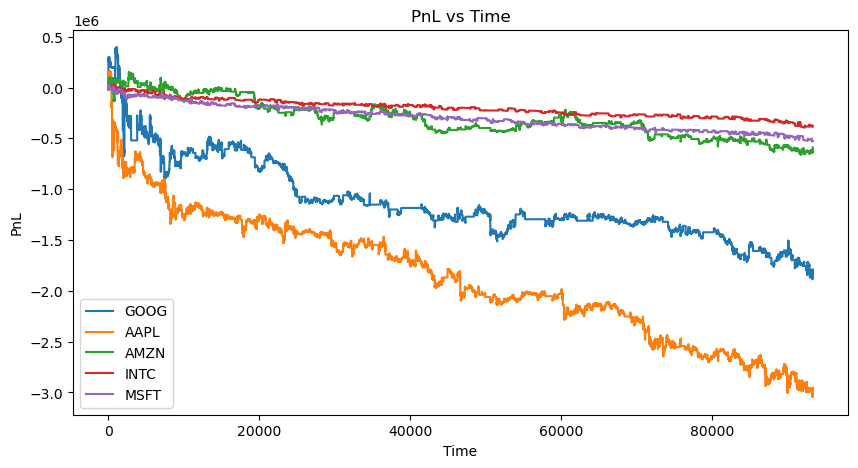
\includegraphics[width=0.5\textwidth]{pnl.png}
\caption{PnL over Time}
\label{fig:pnl}
\end{figure}


Firstly, it is important to mention that the lack of profitability was not unexpected. The Avellaneda-Stoikov strategy, at its core, is a theoretical model developed under certain assumptions which may not necessarily hold in real-world trading environments. For instance, the model assumes a symmetric order flow and infinite liquidity, conditions that are rarely met in reality. It doesn't account for transaction costs, which can significantly impact the profitability of a strategy, especially in high-frequency trading. Additonally, the model requires extensive parameter tuning to achieve optimal performance, which we didn't have time to perform, given the time constraints of this project. Lastly, our model recieved updates in 0.25s timeframes, which is a relatively long time interval for high-frequency trading.   

Despite these limitations, our simulation has provided valuable insights and yielded positive outcomes in several ways:
\begin{enumerate}
        \item \textbf{Effective Inventory Management:} Our model effectively managed inventory risk by maintaining the inventory close to zero throughout the trading day. This is a significant achievement as it minimizes the market maker's exposure to price risk.
        \item \textbf{Realistic Market Dynamics:} The simulated trading activity successfully mirrored realistic market dynamics, validating our approach to modeling the limit order book and market order arrivals.
        \item \textbf{Robustness to Market Conditions:} The Avellaneda-Stoikov strategy demonstrated robustness in a variety of market conditions, adjusting bid-ask prices dynamically in response to changes in the market.
        \item \textbf{MDP Framework:} Our implementation of the Avellaneda-Stoikov strategy as a Markov Decision Process provides a flexible framework for modeling market making strategies and evaluating their performance under realistic market conditions.
\end{enumerate}

Our inventory management results show that we were able to maintain a relatively stable inventory position throughout the trading day. The distribution of inventory for MSFT is shown in Figure \ref{fig:msft_inventory}.

\begin{figure}[h]
\centering
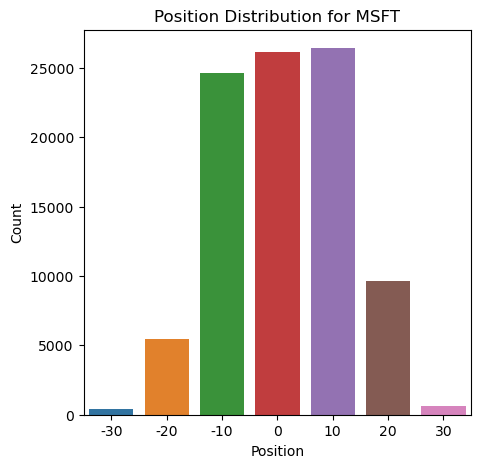
\includegraphics[width=0.5\textwidth]{msft_inventory.png}
\caption{Inventory distribution for MSFT}
\label{fig:msft_inventory}
\end{figure}


In conclusion, while our model did not result in a net profit, it successfully demonstrated the utility of the Avellaneda-Stoikov strategy in managing inventory risk and understanding the intricacies of high-frequency market making. The positive outcomes derived from this research extend far beyond mere profitability and shed light on the complex dynamics of algorithmic trading. This work lays the groundwork for future research aimed at developing more sophisticated market-making strategies that can adapt to real-world trading conditions and transaction costs.


\section{DISCUSSION}

Our project aimed to implement and assess the Avellaneda-Stoikov market making strategy in a high-frequency trading environment using a Markov Decision Process model. The simulation's outcome provided substantial insights into the complexities and challenges of algorithmic market making.

The lack of profitability in our model can be attributed to several factors, including the underlying assumptions of the Avellaneda-Stoikov strategy and the exclusion of transaction costs in our model. The real-world trading environment often deviates from these idealized conditions, leading to discrepancies between theoretical predictions and actual outcomes. For example, real-world market makers also make a fee for simply providing liquidity, and are able to hedge their trades against an ETF, which we didn't account for in our model. 

The key objective of market making is not merely to generate profit but also to provide liquidity and manage inventory risk effectively. Our model demonstrated substantial success in these aspects. The model consistently maintained the inventory close to zero and dynamically adjusted bid-ask prices in response to market conditions to provide liquidity. 

Moving forward, there is considerable scope for refining and extending this work. For instance, incorporating transaction costs and hedging into the model along with reduced times between updates can provide a more realistic representation of trading environments. Additionally, exploring machine learning approaches to model order arrival rates and market dynamics could potentially enhance the adaptability and performance of the market making strategy.

In conclusion, this project contributes to the growing body of research in algorithmic trading and market microstructure. It underscores the importance of effective inventory management in market making and highlights the challenges associated with implementing theoretical trading strategies in real-world markets. Our project has opened doors to future research aimed at developing more sophisticated and adaptive market-making strategies.


\section{CONCLUSION}

% \section*{APPENDIX}

The realm of high-frequency trading and market making is a complex and challenging landscape that necessitates sophisticated strategies and models for successful navigation. Our model of the Avellaneda-Stoikov strategy as a Markov Decision Process demonstrates its potential to manage inventory risk and adapt to dynamic market conditions.

While our simulation did not yield profitability, it revealed the intricacies of market microstructure and the practical challenges of implementing theoretical models in real-world trading environments. This investigation has demonstrated the importance of strategies going beyond mere profit generation and focusing on managing risk, providing liquidity, and effectively responding to market dynamics.

The insights gained from this project will be useful for the development of future market making strategies. By incorporating more realistic market conditions and factors such as transaction costs, and by leveraging advanced machine learning techniques, we can potentially enhance the performance and adaptability of these strategies.

This study is a stepping stone towards a deeper understanding of algorithmic trading and its challenges. It opens up avenues for further research in this domain, with the ultimate goal of creating robust, adaptive, and efficient market-making strategies that can thrive in the rapidly evolving world of high-frequency trading.

\begin{thebibliography}{99}

\bibitem{c1} Stoll, H., 1978, The supply of dealer services in securities markets, Journal of Finance 33, 1133-1151.
\bibitem{c2} Garman M., 1976, Market microstructure, Journal of Financial Economics 3, 257-275.
\bibitem{c3} Ho, T., and Stoll, H., 1981, Optimal dealer pricing under transactions and return uncertainty, Journal of Financial Economics 9, 47-73.
\bibitem{c4} Glosten, L., and Milgrom, P., 1985, Bid, ask and transaction prices in a specialist market with heterogeneously informed traders, Journal of Financial Economics 14, 71-100.
\bibitem{c5} Avellaneda M., and Stoikov S., 2008, High-frequency trading in a limit order book, Quantitative Finance 8, 217-224.
% cite lobsterdata.com 
\bibitem{c6} Lobster Data, https://lobsterdata.com/info/DataSamples.php 



% \bibitem{c3} https://math.nyu.edu/~avellane/HighFrequencyTrading.pdf
\end{thebibliography}




\end{document}
